\documentclass[10pt, a4paper]{amsart}
%\usepackage[english,norsk]{babel}
\usepackage[english]{babel}
\usepackage[utf8]{inputenc}

\usepackage{geometry}   % Margins
\usepackage{graphicx}   % Images
\usepackage{float}      % Image floating
\usepackage{siunitx}    % SI-units
\usepackage{amsmath}
\usepackage[boxed]{algorithm2e}
\usepackage{verbatim}
\usepackage{url}
\usepackage{hyperref}
\usepackage{listings}
\usepackage{framed}
\numberwithin{figure}{section}
\numberwithin{table}{section}
\bibliographystyle{plain}

\usepackage{color}
%\usepackage{multicol}
%\setlength\columnsep{14pt}

\definecolor{codegreen}{RGB}{0, 146, 146}
\definecolor{codegray}{rgb}{0.4,0.4,0.4}
\definecolor{codeblue}{RGB}{0, 109, 219}
\definecolor{backcolour}{rgb}{0.9,0.9,0.9}

\lstdefinestyle{mystyle}{
    backgroundcolor=\color{backcolour},
    commentstyle=\color{codegreen},
    keywordstyle=\color{magenta},
    numberstyle=\tiny\color{codegray},
    stringstyle=\color{codeblue},
    basicstyle=\footnotesize,
    breakatwhitespace=false,
    showstringspaces=false,
    breaklines=true,
    captionpos=b,
    keepspaces=true,
    numbers=left,
    numbersep=5pt,
    showspaces=false,
    basicstyle=\footnotesize \ttfamily \color{black} \bfseries,
    xleftmargin=0.4cm,
    frame=tlbr, framesep=0.1cm, framerule=0pt,
    showtabs=false,
    tabsize=2
}

\lstset{style=mystyle}


\title[Image Denoising]{IN3200 - Project \\ \large
Image Denoising}
\author[Candidate no. 15229]{Candidate no. 15229 \\ \\ \today}


\begin{document}

\maketitle

%\begin{center}
%    Source code can be found in GitHub repository at \url{https://github.com/ejhusom/IN3200/IN3200_PE_ejhusom}
%\end{center}

\tableofcontents

%\begin{multicols}{2}
\section{Introduction}
The goal of this project was to implement an algorithm for denoising images. The project consists of two parts, one with a serial implementation of the algorithm and one parallelized version. For the latter version I used MPI (Message Passing Interface) to parallelize the code.

\section{Program structure}

\subsection{Common functions}

Both the serial and parallel version of the code shares most of the functions:
\begin{itemize}
    \item \texttt{import\_JPEG\_file()} and \texttt{export\_JPEG\_file()}, from the \texttt{simple-jpeg}-library, which imports and exports jpg-files to and from the program.
    \item \texttt{allocate\_image()} and \texttt{deallocate\_image()}, which allocates and deallocates memory to hold the image information in a \texttt{struct} of the type \texttt{image}.
    \item \texttt{convert\_jpeg\_to\_image()} and \texttt{convert\_image\_to\_jpeg()} handles the conversion from jpeg to arrays containing the image information.
\end{itemize}


\subsection{Serial implementation}

The serial version implements the denoising algorithm in the function called \texttt{iso\_diffusion\_denoising()}, and timing measurement is done in the \texttt{main()} function.

\subsection{Parallell implementation}

The parallellized version uses MPI, and the denoising algorithm is contained in the function \texttt{iso\_diffusion\_denoising\_parallel()}. In the \texttt{main()} function the image is distributed on all processes, as evenly as possible. The image is split horisontally, as shown in figure \ref{fig:image_division}. I chose this labour division to make the communication between processes less complex. If the number of elements in the picture is not divisible on the number of processes, the remainder is distributed on all processes except the last one, which means that only one process has a smaller amount of image elements than the others, while the others have an equal amount of elements.

\begin{figure}
    \includegraphics[scale=0.3]{image_division.png}
    \caption{An example of the division of an image with 4 processes. The processes are numbered from 0 to 3.}
    \label{fig:image_division}
\end{figure}

In the \texttt{iso\_diffusion\_denoising\_parallel()} function, each process sends the boundaries (or boundary, in the case of the processes with lowest and highest rank), to the bordering processes, in order to compute the denoising for the complete interior of the picture. To avoid deadlock in this send/recieve-process, I have used a series of \texttt{if}-tests to make even-numbered processes start with sending, and odd-numbered processes start with recieving. After all boundaries/edges have been shared between neighbouring processes, the denoising algorithm is implented.


\section{Example image}

An example of a denoised image is presented in figure \ref{fig:example}.

\begin{figure}
    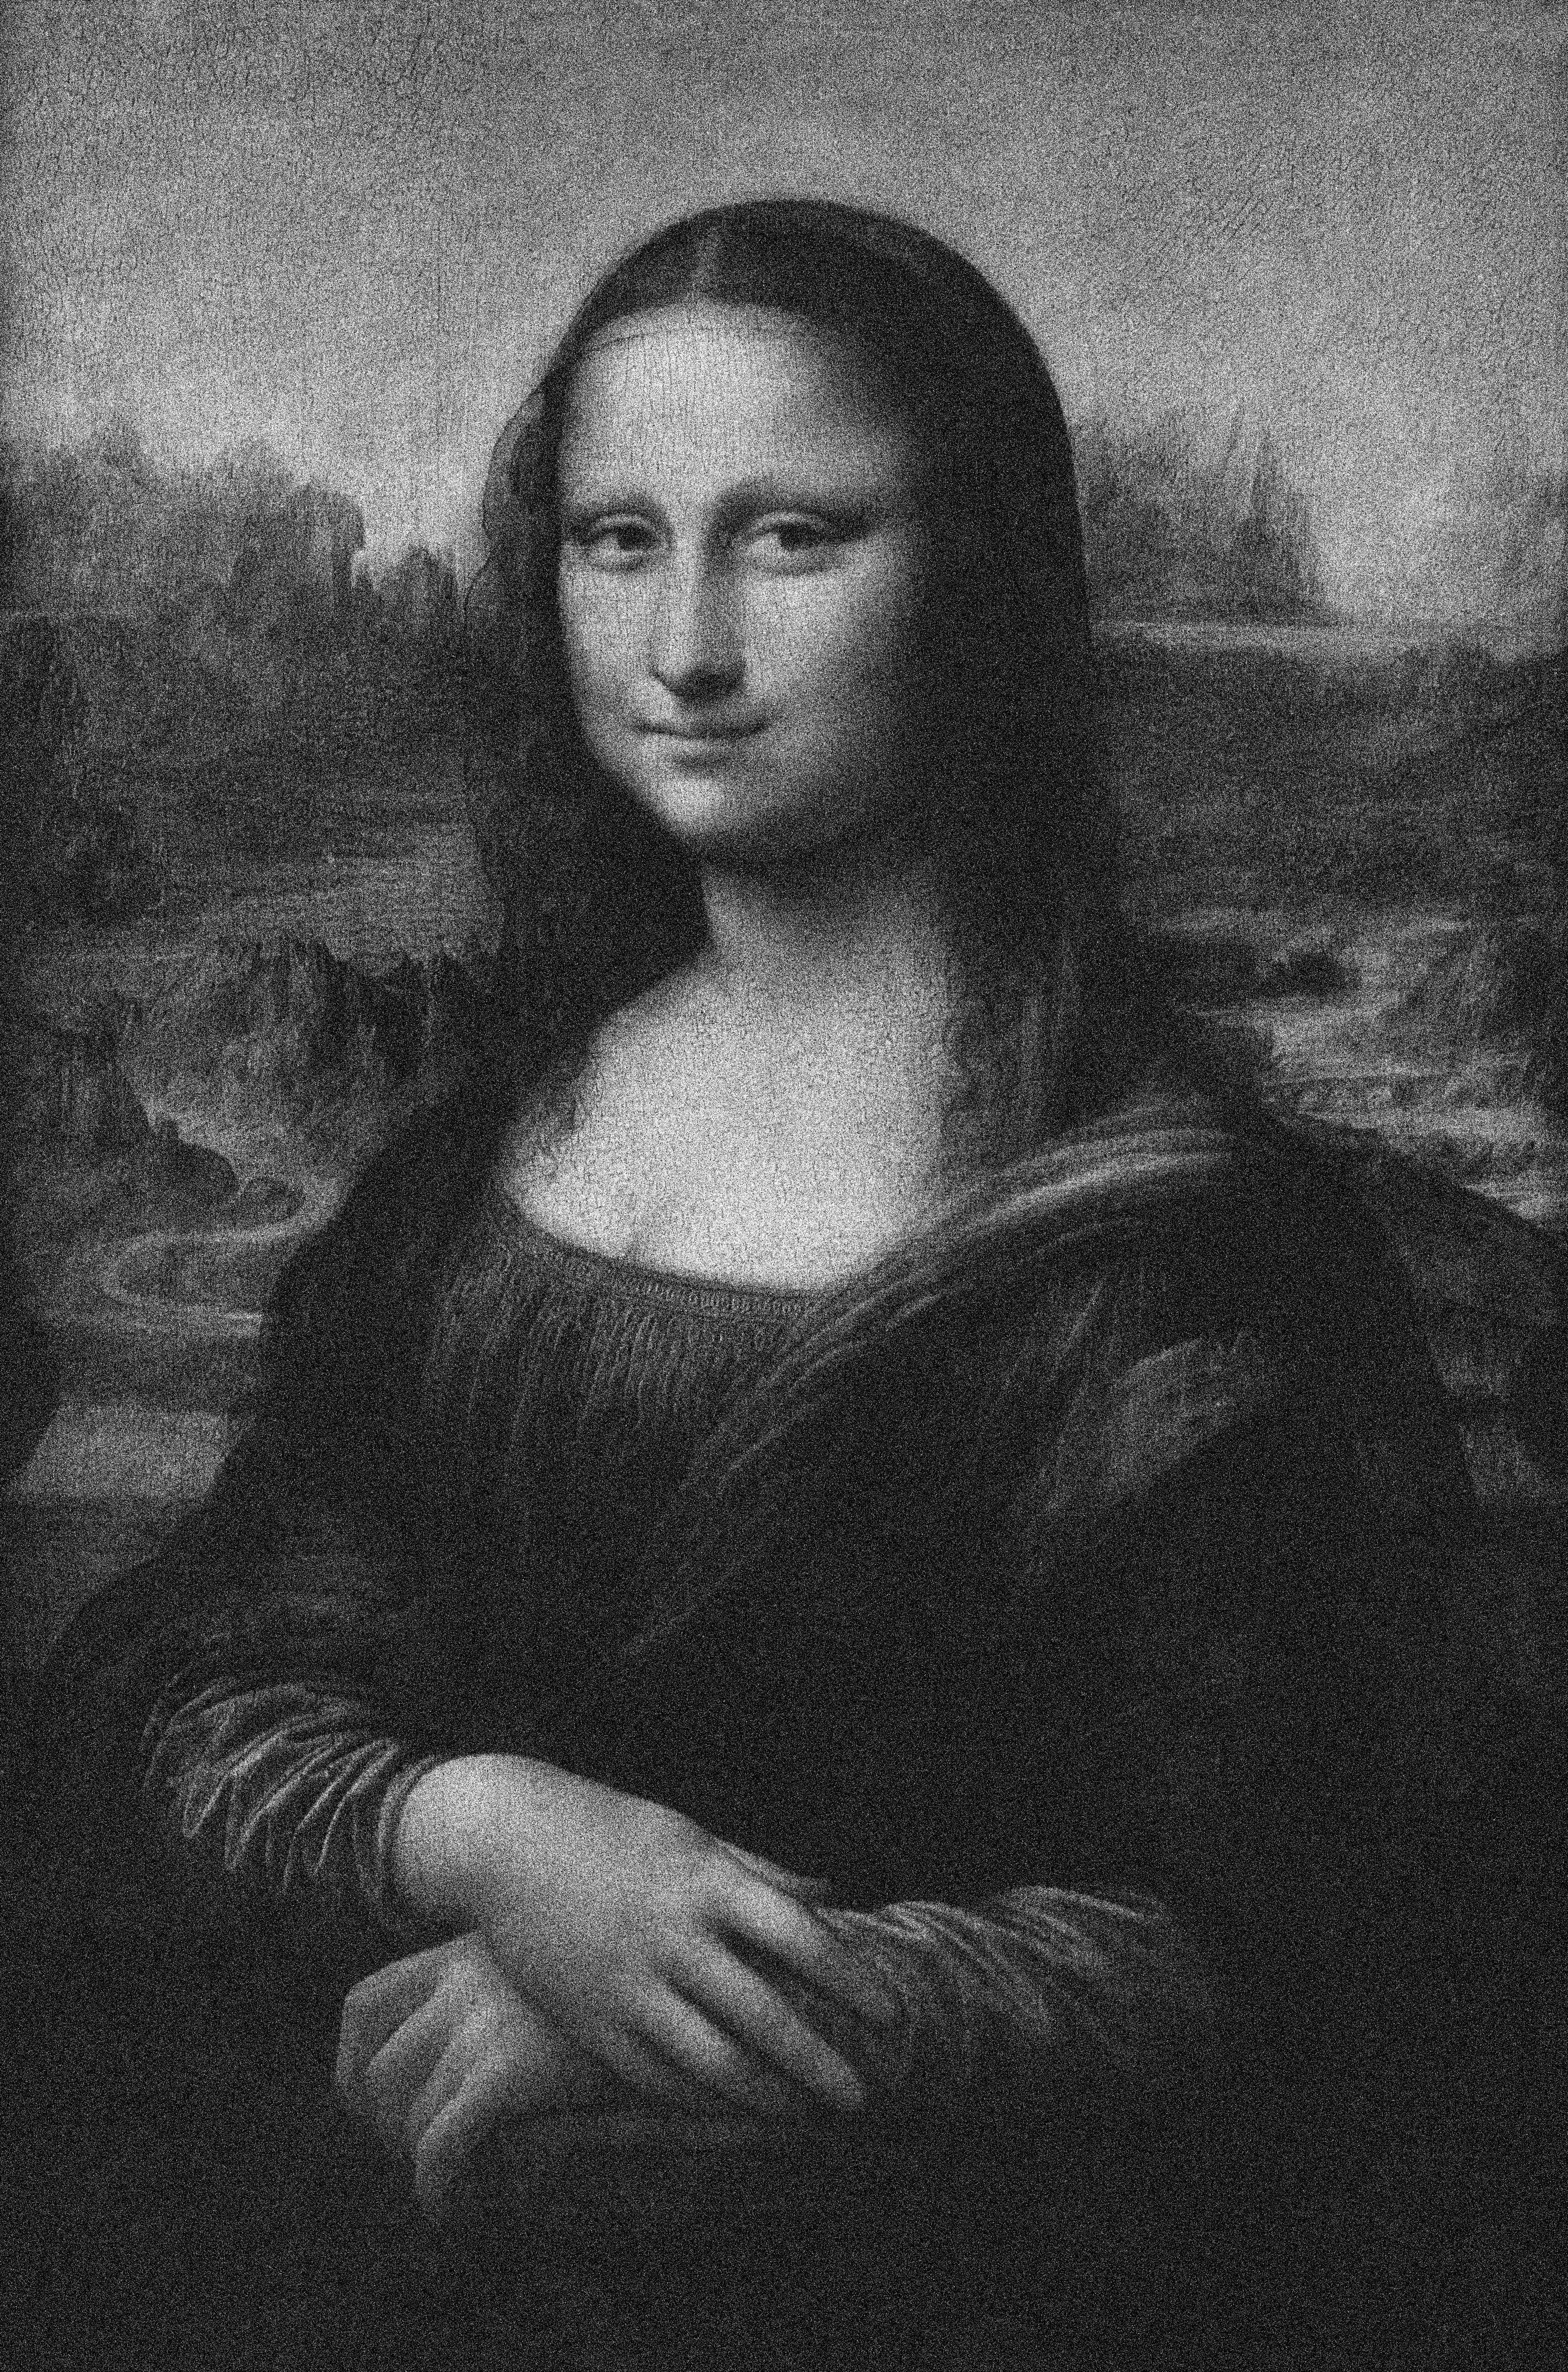
\includegraphics[scale=0.03]{mona_lisa_noisy.jpg}
    \includegraphics[scale=0.03]{denoised_200.jpg}
    \caption{Example of results of image denoising with $\kappa=0.2$ and 200 iterations. Left: Original, noisy image. Right: Denoised image.}
    \label{fig:example}
\end{figure}

\section{Time measurements}
In this section I will present time measurements of the diffusion functions of both the serial and parallel code. All measurements are done with $\kappa=0.2$ and 100 iterations. The hardware used is the following:
\begin{itemize}
  \item Processor: Intel Core M-5Y71 CPU @ 1.20GHz $\times$ 4
  \item Memory: 8 GB DDR3L SDRAM @ 1600 MHz - PC3L-12800
\end{itemize}
The program was run on Ubuntu 18.04 with the C compiler \texttt{gcc}, version 7.3.0.

The time measurements for the parallelized version as a function of number of processes is shown in figure \ref{fig:runtime}. The measurements are done only on the diffusion algorithm itself. I also tested the difference between the optimization flags \texttt{-O2} and \texttt{-O3}, which are used during the compilation of the program.  The latter one contains even more optimization than the former, but increases the compilation time\footnote{According to the \texttt{gcc} documentation: \url{https://gcc.gnu.org/onlinedocs/gcc/Optimize-Options.html}.} As we can see, it is the \texttt{-O3} flag that gives the best performance. According to this analysis, the optimal number of MPI processes is 2. The computer I used has 2 cores with 2 threads on each, in total 4 threads. When using OpenMP, as we did in the partial exam of IN3200 earlier this spring, the best result happened when using 4 processes, one on each thread. In this project, where we use MPI, it seems not to be the case. The measurements have a fairly high degree of uncertainty, because the performance was easily affected by the heat generation of the processor.

Furthermore, we can see from figure \ref{fig:runtime} that the increase in performance from serial to parallel version of the code was quite small when running with the \texttt{-O3} flag. I expected a higher increase in performance, so there might be some problem with the implementation of the parallelized code, for example because of the much overhead. There may be a larger difference when dealing with larger images, when the diffusion of the images is even more demanding than the communication between processes.

\begin{figure}
    \includegraphics[scale=0.9]{../runtime.pdf}
    \caption{Time measurements of the diffusion algorithm, as a function of the numbers of processes. The measurements are averaged over 10 runs per each number of processes, with 200 iterations and $\kappa=0.2$. Two different optimization flags were tested.}
    \label{fig:runtime}
\end{figure}

% \begin{table}
%     \caption{Average time usage of serial code and lowest time usage of parallel code.}
%     \label{tab:time}
%     \begin{tabular}{ll}
%         Function   & Time usage [s] \\
%         \hline
%         \texttt{iso\_diffusion\_denoising()} & \\
%         \texttt{iso\_diffusion\_denoising\_parallel()} & \\
%     \end{tabular}
% \end{table}

% \subsection{Comparison of compiler flags}
%
% In order to optimize the code, I experimented with different compiler flags. The results are shown in table \ref{tab:flags}, and show that the \texttt{O4}-flag gave the best results.
%
% \begin{table}
%     \caption{Comparison of different compiler flags. Time measurements are averaged over 10 runs.}
%     \label{tab:flags}
%     \begin{tabular}{lll}
%         Function   & Time usage for \texttt{iso\_diffusion\_denoising()} [s] & Time usage for \texttt{iso\_diffusion\_denoising\_parallel()} [s] \\
%         \hline
%         O2 & 3.053919 & \\
%         O3 & & \\
%         O4 & & \\
%     \end{tabular}
% \end{table}

\bibliographystyle{unsrt}
\bibliography{references}


%\end{multicols}
\end{document}
